\chapter{Sistemi Attivi Complessi}
In questo capitolo vengono presentate definizioni e modelli che descrivono i sistemi attivi complessi, visti come estensione dei sistemi attivi tradizionali descritti precedentemente. Un sistema attivo complesso è una gerarchia di sistemi attivi tra loro comunicanti. Questo modello si ispira a molti sistemi naturali, fisici, economici e sociali, dei quali è possibile fornire un modello stratificato, in base a diversi livelli di astrazione. Nei sistemi biologici, ad esempio, il comportamento può essere descritto a basso livello dalle interazioni fra le cellule, oppure ad un livello più alto tra i tessuti, o ancora in maniera più astratta studiando il funzionamento degli organi. Nell'ambito dei linguaggi di programmazione a oggetti, ad esempio, a basso livello vi sono le singole istruzioni, a livello più alto i metodi, ad un più alto livello ancora le classi e le interfacce. 
L'attributo ``complesso'' si riferisce, più che alla quantità di componenti presenti nel sistema (che comunque possono essere molti), all'organizzazione gerarchica e alla conseguente stratificazione del comportamento globale del sistema.
Ogni livello della gerarchia di sistemi siffatti ha una evoluzione indipendente dagli altri, eccetto alcune informazioni che giungono dai livelli sottostanti. Ogni livello, in altre parole, ha un comportamento emergente che è impredicibile dalla semplice conoscenza del comportamento dei singoli componenti. Queste informazioni che giungono ai livelli superiori sono rese nel modello dei sistemi attivi complessi attraverso pattern event, che si verificano quando determinate configurazioni delle transizioni dei componenti sottostanti si verificano, soddisfacendo particolari espressioni regolari.

\newpage
\section{Definizioni}
Un sistema attivo complesso (SAC) è una gerarchia di sistemi attivi. In un SAC, vi sono due tipi di comunicazione: tra componenti dello stesso sistema attivo e tra differenti sistemi attivi. 
I componenti di un sistema attivo interagiscono tra loro in base a determinati eventi che giungono o da componenti adiacenti (eventi interni), o da altri sistemi attivi collegati (pattern event) o dal mondo esterno al sistema (eventi esterni). Questi eventi innescano delle transizioni nei componenti, le quali a loro volta generano nuovi eventi, formando una sequenza di transizioni detta traiettoria del SAC.
Analogamente ai sistemi attivi tradizionali, un sistema attivo complesso può essere in uno stato quiescente, nel quale nessun evento si verifica e conseguentemente non vengono innescate transizioni dei componenti.
Il SAC diviene reattivo nel momento in cui si verifica un evento esterno che può essere consumato da un componente. In tale circostanza la transizione di un componente modifica lo stato del sistema, dove lo stato è caratterizzato dalla composizione di tutti gli stati dei componenti, dagli eventi non ancora consumati presenti nei terminali di input, e dagli stati relativi agli automi (pattern space) responsabili del matching delle espressioni regolari generanti i pattern event. 

\subsection{Nodi}
Un sistema attivo complesso è composto da un insieme di sistemi attivi che interagiscono tra loro. Ogni singolo sistema attivo è detto nodo, in quanto costituisce un nodo nella gerarchia che costituisce la topologia del sistema.
Il modello di un nodo, a cui più istanze di nodi possono fare riferimento, possiede tutti gli attributi di un sistema attivo, con l'aggiunta di alcuni elementi:
\begin{itemize}
\item un insieme $I$ di terminali di input, nei quali giungono pattern event generati da nodi del livello inferiore;
\item un insieme $O$ di terminali di output, nei quali vengono generati i pattern event del nodo corrente, che vengono inviati a uno o più nodi del livello superiore;
\item un insieme $P$ di dichiarazioni di pattern;
\item un insieme $L_{patt}$ di link uscenti da terminali di input del nodo ed entranti in terminali di input dei componenti.
\end{itemize}
Quest'ultima caratteristica aggiuntiva consente l'invio dei pattern event in ingresso al nodo ai componenti particolari predisposti a gestire tali eventi.

\subsection{Pattern}
Una dichiarazione di pattern è una quadrupla $(p,l,r,o)$ dove:
\begin{itemize}
\item $p$ è il nome del pattern event;
\item $l$ è il linguaggio relativo al pattern;
\item $r$ è una espressione regolare;
\item $o \in O$ è un terminale di output in corrispondenza del quale il pattern event viene generato.
\end{itemize}
Il linguaggio $l$ del pattern può variare dal linguaggio minimo, cioè costituito dalle sole transizioni facenti parte dell'espressione regolare $r$, al linguaggio massimo, ovvero corrispondente all'insieme di tutte le transizioni di componenti del nodo. L'appartenenza a diversi linguaggi conferisce una semantica differente a quei pattern le cui espressioni regolari utilizzano operatori insiemistici, come ad esempio il $not$. Si nota facilmente che il complemento di una transizione rispetto a linguaggi differenti ha come risultato una unione di transizioni che, data l'operazione di complemento applicata su insiemi diversi, varia.

\subsection{Link tra nodi}
Un sistema attivo complesso, oltre che da un insieme di nodi, è caratterizzato dalla topologia con cui i nodi sono collegati tra loro. Si assume che tale topologia generi un albero.
I nodi sono tra loro connessi per mezzo di link. I link tra nodi sono definiti analogamente ai link tra componenti del singolo sistema attivo, con la differenza che i primi connettono tra loro sistemi attivi.
In un SAC ogni link esce da un terminale di output $o$ di un nodo $n$ e entra in un terminale di input $i$ di un nodo $n^\prime$.
I link sono caratterizzati da un modello, che costituisce un'astrazione del link specifico in esame.

\begin{defn}
Un modello di un link è una quadrupla
\begin{center}
	$M_{l_c} = (i,o,z,w)$
\end{center}
dove $i$ è il terminale di input, $o$ il terminale di output, $z$ la dimensione e $w$ la politica di saturazione.
\end{defn}
Un particolare link $l_c$ è un'istanza di un modello siffatto, e consiste quindi in un canale di comunicazione unidirezionale fra due nodi del sistema $n$ e $n^\prime$, dove un terminale di output $o$ di $n$ e un terminale di input $i$ di $n^\prime$ coincidono rispettivamente con l'input e l'output del link $l_c$.
La dimensione $z$ rappresenta il numero massimo di eventi che possono essere accodati nel link. 
Indichiamo con $|l_c|$ la configurazione corrente del link. 
Se il numero di eventi attualmente memorizzati coincide con la dimensione, il link si dice essere saturo.
Quando il link è saturo, la semantica legata al compimento delle transizioni è dettata dalla politica di saturazione $w$ (si veda il paragrafo \ref{saturation}).
Come per i link tra componenti, anche per quanto riguarda i link tra nodi, nel seguito della trattazione, si farà riferimento al caso in cui la dimensione sia unitaria e la politica di saturazione sia $wait$.

\begin{ex} \label{ex:ref}
Si consideri l'esempio di sistema attivo complesso riportato in figura \ref{fig:sac}. Esso consiste in una linea elettrica. Ogni capo della linea è protetto dai cortocircuiti per mezzo di due breaker, $b_1$ e $r_1$ da un lato, e $b_2$ e $r_2$ dall'altro. Sia $b_1$ che $b_2$ sono connessi ad una protezione che rileva bassa tensione. Se uno dei due sensori rileva un imminente cortocircuito, comanda l'apertura del breaker collegato. Se tutti e due i breaker si aprono, il cortocircuito si estingue e successivamente la chiusura dei breaker permette di ripristinare la linea. Tuttavia possono verificarsi dei guasti: o la protezione invia il comando sbagliato, oppure il breaker non si apre. Questi malfunzionamenti sono rilevati da un monitor (uno per ogni capo della linea), che in caso di non apertura del breaker ne comanda uno di emergenza, $r_1$ e $r_2$ rispettivamente per il monitor $m_1$ e $m_2$. Nel compiere questa azione, inoltre, il monitor informa l'altro monitor di effettuare la medesima operazione. Si assume che i breaker di emergenza, per ragioni di sicurezza, non vengano chiusi nuovamente. Il SAC dell'esempio possiede quattro nodi:
\begin{itemize}
\item l'organo di protezione $W_1$, che include la protezione $p_1$ e il breaker $b_1$;
\item l'organo di protezione $W_2$, che include la protezione $p_2$ e il breaker $b_2$;
\item l'apparato monitor $M$, che include i monitor $m_1$ e $m_2$, oltre ai breaker di emergenza $r_1$ e $r_2$;
\item il nodo radice $L$, che contiene il componente $l$, il quale rappresenta l'intera linea elettrica.
\end{itemize}
I nodi $W_1$ e $W_2$ condividono lo stesso modello di nodo, hanno cioè gli stessi terminali, gli stessi componenti e le medesime dichiarazioni di pattern.
Le frecce in figura all'interno del singolo nodo rappresentano link tra componenti o link tra terminali di input del nodo e terminali di input di componenti (per la gestione dei pattern event). I link tra i nodi rappresentano le interazioni tra sistemi attivi, che avvengono tramite la generazione di pattern event da nodi inferiori verso i nodi superiori della gerarchia.
I componenti di protezione condividono il modello in figura \ref{fig:model_p}, mentre i breaker hanno il medesimo modello in figura \ref{fig:model_b}. I monitor $m_1$ e $m_2$ hanno un comportamento descritto in figura \ref{fig:model_m}, mentre la linea $l$ è rappresentata in figura \ref{fig:model_l}.
Le transizioni relative alle protezioni e ai breaker sono fornite rispettivamente nelle tabelle \ref{tab:p_trans} e \ref{tab:b_trans}, mentre le transizioni dei monitor e della linea sono nelle tabelle \ref{tab:m_trans} e \ref{tab:l_trans}. Si noti che i pattern event sono indicati in grassetto.
Nella tabella \ref{tab:pattern_w} sono riportate le dichiarazioni di pattern condivise dai nodi $W_1$ e $W_2$. 
Nella tabella \ref{tab:pattern_m} vi sono i pattern relativi all'apparato monitor $M$.
Si noti che non è specificato il terminale di output in corrispondenza del quale il pattern event viene generato, in quanto si assume che ogni nodo abbia un unico terminale di uscita. Il nodo $M$ possiede inoltre due terminale di input, sui quali riceve i pattern event dei nodi $W_1$ e $W_2$ rispettivamente.
I linguaggi dei pattern sono così definiti:
\begin{itemize}
\item per $W_1$ e $W_2$ il linguaggio è massimo e l'alfabeto coincide con l'intero insieme di transizioni dei componenti del nodo;
\item per $M$ il linguaggio è minimo e l'alfabeto di ogni pattern coincide con le uniche transizioni coinvolte nella relativa espressione regolare (i tre pattern specificati hanno dunque tre linguaggi diversi).
\end{itemize}
\end{ex}

\begin{figure}[htbp]
\centering
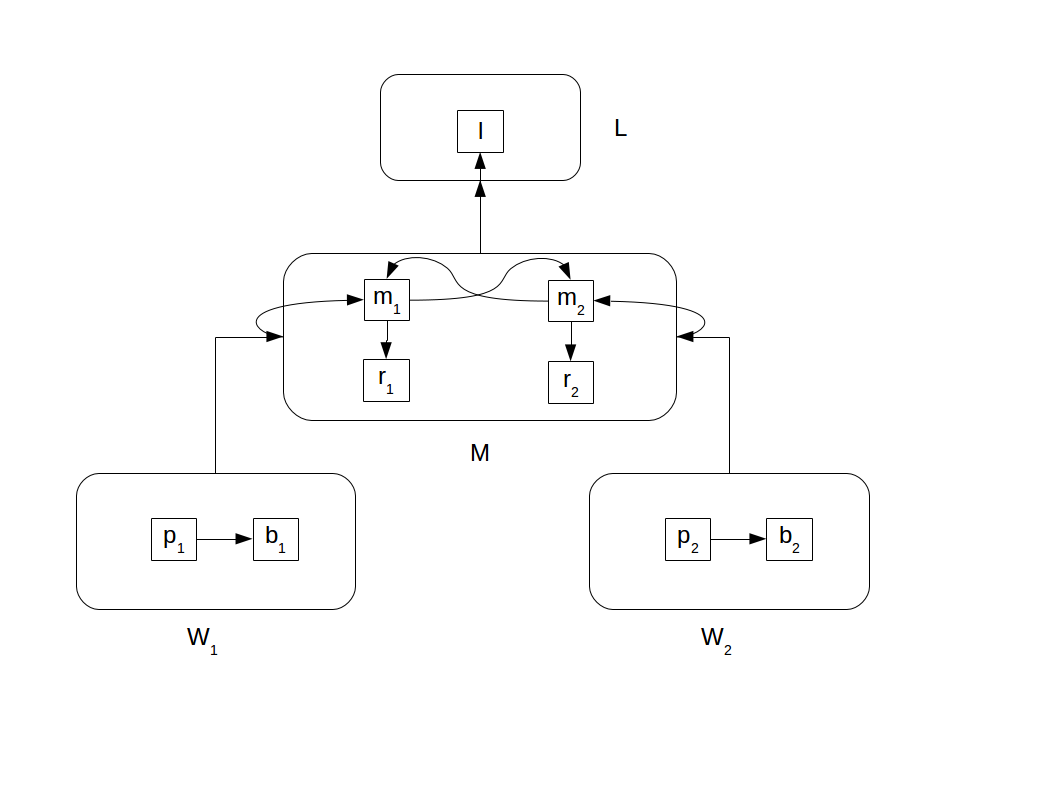
\includegraphics[scale=0.4]{./Img/sac/sac.png}
\caption{Esempio di riferimento}
\label{fig:sac}
\end{figure}

\begin{figure}[htbp]
\centering
\subfigure[topologia monitor]
{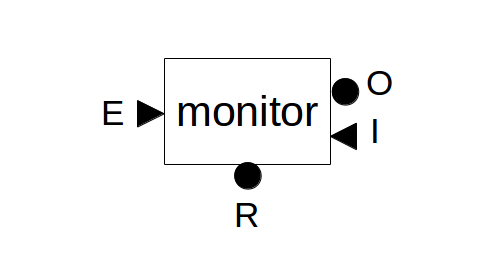
\includegraphics[scale=0.4]{./Img/sac/top_monitor.png}}
\hspace{10mm}
\subfigure[comportamento monitor]
{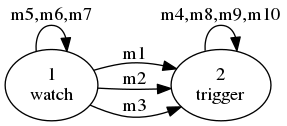
\includegraphics[scale=0.5]{./Img/sac/model_monitor.png}}
\caption{Modello dei componenti $m_1$ e $m_2$}
\label{fig:model_m}
\end{figure}

\begin{figure}[htbp]
\centering
\subfigure[topologia linea]
{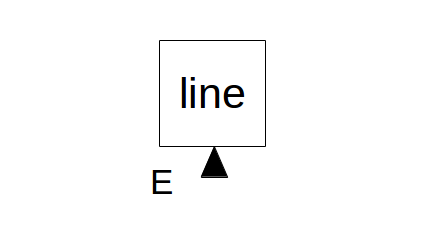
\includegraphics[scale=0.4]{./Img/sac/top_line.png}}
\hspace{10mm}
\subfigure[comportamento linea]
{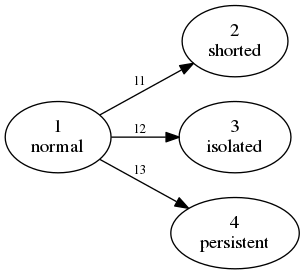
\includegraphics[scale=0.5]{./Img/sac/model_line.png}}
\caption{Modello del componente $l$}
\label{fig:model_l}
\end{figure}

\begin{table}[htbp] 
\begin{tabularx}{\textwidth}{l X}
\hline
\textbf{Transizione} & \textbf{Descrizione}\\
\hline\\
$m_1 = watch \xrightarrow{(\textbf{nd},E) \Rightarrow \{(op,R),(rc,O)\}} trigger$ & Rileva la mancata disconnessione del lato della linea e comanda l'apertura del breaker di emergenza, informando l'altro monitor\\[1mm]
$m_2 = watch \xrightarrow{(\textbf{nd},E) \Rightarrow (op,R)} trigger$ & Rileva la mancata disconnessione del lato della linea e comanda l'apertura del breaker di emergenza\\[1mm]
$m_3 = watch \xrightarrow{(rc,I) \Rightarrow (op,R)} trigger$ & Riceve il messaggio dell'altro monitor e comanda l'apertura del proprio breaker\\[1mm]
$m_4 = trigger \xrightarrow{(\textbf{nd},E)} trigger$ & Consuma il pattern event $\textbf{nd}$\\[1mm]
$m_5 = watch \xrightarrow{(\textbf{di},E)} watch$ & Consuma il pattern event $\textbf{di}$\\[1mm]
$m_6 = watch \xrightarrow{(\textbf{co},E)} watch$ & Consuma il pattern event $\textbf{co}$\\[1mm]
$m_7 = watch \xrightarrow{(\textbf{nc},E)} watch$ & Consuma il pattern event $\textbf{nc}$\\[1mm]
$m_8 = trigger \xrightarrow{(\textbf{di},E)} trigger$ & Consuma il pattern event $\textbf{di}$\\[1mm]
$m_9 = trigger \xrightarrow{(\textbf{co},E)} trigger$ & Consuma il pattern event $\textbf{co}$\\[1mm]
$m_{10} = trigger \xrightarrow{(\textbf{nc},E)} trigger$ & Consuma il pattern event $\textbf{nc}$\\[1mm]
\hline
\end{tabularx}
\caption{Transizioni relative al monitor}
\label{tab:m_trans}
\end{table}

\begin{table}[htbp] 
\begin{tabularx}{\textwidth}{l X}
\hline
\textbf{Transizione} & \textbf{Descrizione}\\
\hline\\
$l_1 = normal \xrightarrow{(ni,E)} shorted$ & Consuma il pattern event $\textbf{ni}$\\[1mm]
$l_2 = normal \xrightarrow{(nr,E)} isolated$ & Consuma il pattern event $\textbf{nr}$\\[1mm]
$l_3 = normal \xrightarrow{(ps,E)} persistent$ & Consuma il pattern event $\textbf{ps}$\\[1mm]
\hline
\end{tabularx}
\caption{Transizioni relative alla linea}
\label{tab:l_trans}
\end{table}

\begin{table}[htbp] 
\begin{tabularx}{\textwidth}{l X}
\hline
\textbf{Pattern event} & \textbf{Espressione regolare}\\
\hline\\
$\textbf{di}$ & $b_1(b)$\\[1mm]
$\textbf{co}$ & $b_2(b)$\\[1mm]
$\textbf{nd}$ & $p_3(p) | p_1(p)b_3(b)$\\[1mm]
$\textbf{nc}$ & $p_4(p) | p_2(p)b_4(b)$\\[1mm]
\hline
\end{tabularx}
\caption{Dichiarazioni di pattern dei nodi $W_1$ e $W_2$}
\label{tab:pattern_w}
\end{table}

\begin{table}[htbp] 
\begin{tabularx}{\textwidth}{l X}
\hline
\textbf{Pattern event} & \textbf{Espressione regolare}\\
\hline\\
$\textbf{nr}$ & $m_7(m_1) | m_{10}(m_1) | b_1(r_1) | m_7(m_2) | m_{10}(m_2) | b_1(r_2) $\\[1mm]
$\textbf{ni}$ & $(m_1(m_1) | m_2(m_1) | m_4(m_1))b_3(r_1) | b_3(r_1)m_4(m_1) |$\\
			  &	$(m_1(m_2) | m_2(m_2) | m_4(m_2))b_3(r_2) | b_3(r_2)m_4(m_2)$\\[1mm]
$\textbf{ps}$ & $(m_6(m_1)m_6(m_2) | m_6(m_2)m_6(m_1))$\\
			  & $(m_5(m_1)m_5(m_2) | m_5(m_2)m_5(m_1))$\\[1mm]
\hline
\end{tabularx}
\caption{Dichiarazioni di pattern del nodo $M$}
\label{tab:pattern_m}
\end{table}

\newpage
\subsection{Pattern space}
In modo da individuare pattern event, deve essere mantenuto lo stato relativo al matching dei pattern coinvolti. A tal fine, per ogni nodo, è necessario generare degli automi, chiamati \emph{pattern space}, secondo i seguenti passi:
\begin{itemize}
\item per ogni pattern $(p,l,r,o)$, viene generato un automa deterministico equivalente all'espressione regolare $r$, nel quale ogni stato finale viene marcato dal nome $p$ del pattern event;
\item per ogni linguaggio utilizzato nella definizione dei pattern, vengono identificati i pattern che utilizzano tale linguaggio, corrispondenti agli automi $[A_1, \ldots , A_k]$, e viene generato un pattern space nel seguente modo:
	\begin{enumerate}
	\item un automa non deterministico $N$ è creato generando il suo stato iniziale $s_0$ e una $\epsilon$-			transizione da $s_0$ a ogni stato iniziale di $A_i$, con $i \in [1 \ldots k]$;
	\item in modo da mantenere il matching di stringhe sovrapposte, viene aggiunta una $\epsilon$-transizione	da ogni stato non iniziale a $s_0$;
	\item l'automa $N$ viene determinizzato nel risultante pattern space $Pts$, dove ogni stato finale $s_f$ è marcato dall'unione \textbf{p} dei pattern event associati agli stati in $s_f$ che sono finali nei corrispondenti automi di pattern generati inizialmente. Ogni stato $s$ dell'automa deterministico $Pts$ è infatti identificato da un sottoinsieme di stati dell'automa non deterministico equivalente $N$;
	\item l'automa $Pts$ viene minimizzato, raggruppando tra loro gli stati equivalenti che sono provvisti dello stesso tag (altrimenti l'informazione relativa ai pattern event generati potrebbe andare persa) \footnote{La minimizzazione del pattern space richiede una lieve modifica nella partizione iniziale: oltre a distinguere tra stati finali e stati non finali, si effettua una partizione in base al contenuto del tag degli stati finali}.
	\end{enumerate}
\end{itemize}

\begin{ex}
Viene di seguito presentata la costruzione del pattern space relativo a due pattern(figura\ref{fig:patt_build}).
Siano
\begin{itemize}
\item $p_1 = t_1$
\item $p_2 = t_2$
\end{itemize}
due dichiarazioni di pattern, alle quali corrispondono gli automi $A_1$ e $A_2$, costruiti attraverso la costruzione di Thompson. L'automa NFA $N$ è ottenuto inserendo uno stato iniziale fittizio $s_0$, collegando quest'ultimo agli stati iniziali dei due DFA per mezzo di $\epsilon$-transizioni e collegando ogni stato non iniziale dei due DFA allo stato $s_0$ tramite $\epsilon$-transizioni. La determinizzazione di tale automa risultante è il pattern space $Pts$ per i pattern $p_1$ e $p_2$. Si noti che non è necessaria la minimizzazione.
\end{ex}

\begin{figure}[htbp]
\centering
\subfigure[Automi $A_1$ e $A_2$]
{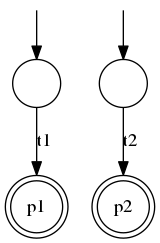
\includegraphics[scale=0.5]{./Img/sac/a1_a2.png}}
\hspace{10mm}
\subfigure[NFA $N$]
{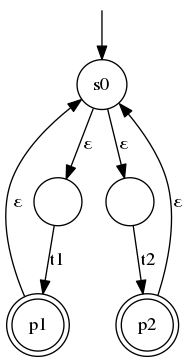
\includegraphics[scale=0.4]{./Img/sac/N.png}}
\hspace{10mm}
\subfigure[Pattern space]
{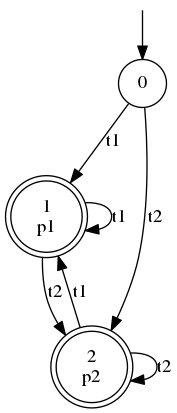
\includegraphics[scale=0.4]{./Img/sac/pts.png}}
\caption{Esempio di costruzione del pattern space}
\label{fig:patt_build}
\end{figure}

\begin{ex}
Specificato in tabella \ref{tab:pts_w} vi è il pattern space relativo ai nodi $W_1$ e $W_2$. Gli stati finali hanno come etichetta i nomi dei relativi pattern riconosciuti.
Per quanto riguarda il nodo $M$, dato che i pattern sono caratterizzati da linguaggi differenti, vengono invece generati tre pattern space distinti.
\end{ex}

\begin{table}[htbp] 
\begin{tabularx}{\textwidth}{X | X X X X X X X X | X}
\hline
 & $b_1$ & $b_2$ & $b_3$ & $b_4$ & $p_1$ & $p_2$ & $p_3$ & $p_4$ & \\
\hline
$0$ & $1$ & $2$ &  &  & $3$ & $4$ & $5$ & $6$ & \\
$1$ & $1$ & $2$ &  &  & $3$ & $4$ & $5$ & $6$ & $\textbf{di}$\\
$2$ & $1$ & $2$ &  &  & $3$ & $4$ & $5$ & $6$ & $\textbf{co}$\\
$3$ & $1$ & $2$ & $5$ &  & $3$ & $4$ & $5$ & $6$ & \\
$4$ & $1$ & $2$ &  & $6$ & $3$ & $4$ & $5$ & $6$ & \\
$5$ & $1$ & $2$ &  &  & $3$ & $4$ & $5$ & $6$ & $\textbf{nd}$\\
$6$ & $1$ & $2$ &  &  & $3$ & $4$ & $5$ & $6$ & $\textbf{nc}$\\
\hline
\end{tabularx}
\caption{Pattern space per i nodi $W_1$ e $W_2$}
\label{tab:pts_w}
\end{table}

\subsection{Sistema attivo complesso}
Un sistema attivo complesso è una rete di nodi interconnessi per mezzo di link. Ogni nodo ed ogni link del sistema sono caratterizzati da un modello e quindi, in generale, più elementi potrebbero avere il medesimo modello. Si assume che più link possano uscire da un terminale di output di un nodo, mentre al massimo un link possa entrare in un terminale di input.

\begin{defn}
Un sistema attivo complesso è una coppia
\begin{center}
	$ C = (N,L_c)$
\end{center}
dove $N$ è l'insieme di nodi, mentre $L_c$ è l'insieme dei link tra terminali di nodi appartenenti a $N$.
\end{defn}


\subsection{Traiettoria}
Un SAC può essere pensato come una macchina che può essere in uno stato quiescente o in uno stato reattivo. Se si trova nello stato quiescente, i componenti non effettuano alcuna transizione, dal momento che nessun evento è disponibile nei terminali di ingresso. In corrispondenza del verificarsi di un determinato evento proveniente dal mondo esterno, il sistema evolve nella sua fase reattiva. Dato che il comportamento del sistema è asincrono (non dipende dal tempo), la reazione, detta traiettoria (o storia), consiste in una sequenza di transizioni compiute da componenti presenti nel sistema.
Ogni transizione di un componente porta il sistema in un nuovo stato, dove uno stato è identificato dallo stato corrente di ogni componente di ogni nodo,dalle configurazioni attuali dei link dei nodi e dallo stato attuale dei pattern space di tutti i nodi. Quando un pattern space raggiunge uno stato finale, il relativo pattern event viene inviato al terminale corrispondente.
In altre parole, uno stato del sistema attivo complesso è una tripla $(S,Q,Pts)$, dove $S$ è la n-pla degli stati dei componenti dei nodi, $Q$ è la m-pla delle configurazioni dei link tra nodi, mentre $Pts$ è la p-pla di pattern space di tutti i nodi.
Quindi una transizione del sistema può essere scritta come:
\begin{center}
	$T = (S,Q,Pts) \xrightarrow {t(c(n))} (S^\prime,Q^\prime,Pts^\prime)$,
\end{center}
dove $t(c(n))$ identifica univocamente la transizione $t$ appartenente al modello del componente $c$ nel nodo $n$.
Assumendo che $a_0 = (S_0,Q_0,Pts_0)$ sia lo stato iniziale del sistema, la traiettoria ottenuta partendo da $a_0$ è la sequenza di stati del sistema determinata dall'occorrenza di transizioni $t_1, \ldots , t_k$ attuabili da parte dei singoli componenti dei nodi:
\begin{center}
$h = a_0 \xrightarrow{t_1(c_1(n_1))} a1 \xrightarrow{t_2(c_2(n_2))} a2 \ldots \xrightarrow{t_k(c_k(n_k))} a_k$.
\end{center}

Ogni stato (non iniziale) dipende quindi dallo stato precedente e dalla particolare transizione che lo porta allo stato corrente, ovvero la coppia $(a_{i-1},t_i(c_i(n_i)))$. Assumendo che si parta dallo stato iniziale $a_0$ questo ci permette di identificare una traiettoria per mezzo delle sole transizioni dei componenti dei nodi:
\begin{center}
$h = [t_1(c_1(n_1)),t_2(c_2(n_2)), \ldots , t_k(c_k(n_k))]$.
\end{center}


\subsection{Behavior space}
Dato un SAC $C$ ed il suo stato iniziale, possono esservi infinite traiettorie, descritte da un automa. 
Quest'ultimo è detto behavior space e ha come alfabeto l'intero insieme delle transizioni dei singoli componenti di ogni nodo.
Il linguaggio del behavior space $Bsp(C)$ con stato iniziale $a_0$ coincide con l'insieme di tutte le possibili traiettorie del sistema $C$ partendo dallo stato $a_0$. 
\begin{defn}
Sia $C = (N,L)$ un sistema attivo complesso, dove $N$ è l'insieme di nodi, mentre $L$ è l'insieme di link tra i nodi. Il behavior space di $C$ è il DFA
\begin{center}
	$Bsp(C) = (\Sigma,\alpha,\tau,a_0)$
\end{center}
dove:
\begin{enumerate}
\item $\Sigma$ è l'alfabeto, dato dall'unione delle transizioni dei componenti di tutti i nodi in $N$;
\item $\alpha$  è l'insieme degli stati $(S,Q,Pts)$, con $S = (s_1,\ldots,s_n)$ una n-pla di stati dei componenti in ogni nodo in $N$, $Q = (q_1, \ldots,q_m)$ una m-pla di configurazioni dei link interni ai nodi in $N$, e $Pts = (pts_1, \ldots, pts_p)$ una p-pla di stati dei pattern space di tutti i nodi in $N$;
\item $a_0 = (S_0,Q_0,Pts_0)$ è lo stato iniziale;
\item $\tau$ è la funzione di transizione deterministica, $\tau: \alpha \times \Sigma \rightarrow \alpha$, tale che 
\begin{center}
$(S,Q,Pts) \xrightarrow{t(c(n))} (S^\prime, Q^\prime, Pts^\prime) \in \tau$,
\end{center}
dove $S = (s_1, \ldots,s_n)$, $Q = (q_1, \ldots,q_m)$, $Pts = (pts_1, \ldots, pts_p)$, $S^\prime = (s^\prime_1, \ldots,s^\prime_n)$, $Q^\prime = (q^\prime_1, \ldots,q^\prime_m)$, $Pts^\prime = (pts_1^\prime, \ldots, pts_p^\prime)$ e
\begin{center}
$t(c(n)) = s \xrightarrow{(e,x) | \{(e_1,y_1), \ldots, (e_p,y_p)\}} s^\prime$
\end{center}
se e solo se:
\begin{itemize}
\item $x = In$, cioè l'evento è disponibile sul terminale di input virtuale sensibile agli eventi esterni al sistema;
\item Per ogni $i \in [1 \ldots n]$, abbiamo
\begin{center}
$s^\prime_i = \begin{cases} s^\prime & \mbox{se }c_i = c\\ s_i & \mbox{altrimenti} \end{cases}$
\end{center}
cioè per ogni transizione del behavior space cambia lo stato relativo al singolo componente coinvolto nella transizione;
\item $Pts^\prime$ differisce d $Pts$ solo negli elementi $w \in [j, \ldots, k]$ corrispondenti a pattern space del nodo $n$ coinvolto nella transizione, secondo il seguente comportamento:
\begin{center}
$Pts^\prime(pts_w) = \begin{cases} \overline{P} & \mbox{se esite}Pts(pts_w) \xrightarrow{t(c(n))} \overline{P}\\ P_{w,0} & \mbox{altrimenti} \end{cases}$;
\end{center}
\item $Q^\prime$ differisce da $Q$ per le seguenti condizioni:
\begin{itemize}
\item $Q(x) = e \rightarrow Q^\prime(x) = \epsilon$, cioè l'evento in input è consumato;
\item $\forall(e_j,y_j), j \in [1 \ldots p], Q(y_j) = \epsilon \rightarrow Q^\prime(y_j) = e_j$, cioè gli eventi di uscita sono inseriti nei terminali di input connessi ai terminali di output coinvolti nella transizione;
\item se $Pts^\prime(pts_w) \neq Pts(pts_w), w \in [j, \ldots, k]$ di pattern space relativi al nodo $n$, $Pts^\prime(P_w)$ è finale e marcato dall'insieme di eventi \textbf{p}, allora ogni $p_i \in \textbf{p}$  ha un terminale destinazione $o_i \in O$ del nodo $n$. Ogni terminale di output di $n$ è collegato ad uno o più terminali di input di un nodo superiore $n^\prime$, che a sua volta è collegato ad uno o più terminali di input $i_z$ che gestiscono il patter event. Per ogni terminale $i_z$, il relativo contenuto passa da $\epsilon$ al pattern event $p_i$.
\end{itemize}
\end{itemize}
\end{enumerate}
\end{defn}

\begin{ex}
Si consideri l'esempio di riferimento \ref{ex:ref}. Si può facilmente notare come una eventuale generazione del behavior space sia impraticabile. La dimensione dell'automa, infatti, è superiormente limitata da tutte le possibili combinazioni di stati dei nodi, contenuto dei terminali di input e stato dei pattern space dell'intero sistema. Dato che il sistema è composto da nove componenti, nove terminali di input e quattro pattern space, considerando anche solo due possibili configurazioni per ogni elemento (in realtà sono molte di più, ad esempio i pattern space dei nodi $W_1$ e $W_2$ hanno sette stati), gli stati possibili sarebbero $2^{22}$, cioè più di quattro milioni. I risultati sperimentali hanno evidenziato una saturazione della memoria (4GB di RAM) per automi di dimensione inferiore ai due milioni.
\end{ex}


\newpage
\section{Problema di diagnosi}
Analogamente al caso di sistemi attivi tradizionali, il problema di diagnosi dei sistemi attivi complessi necessita di informazioni riguardanti l'osservabilità e i guasti delle transizioni dei componenti di ogni nodo. Si suppone sia disponibile, terminata la reazione, l'osservazione riferita ad ogni singolo sistema attivo che compone il sistema. Si ricorda che nell'ambito di questo lavoro ci si focalizza sulla cosiddetta diagnosi a posteriori, ovvero a seguito di una traiettoria completa del sistema, che parte da uno stato iniziale noto quiescente e termina in uno stato finale (sconosciuto a priori) anch'esso quiescente. 

\subsection{Viewer}
Per ogni nodo un viewer locale specifica quali transizioni sono osservabili, associando ad esse una label. Il viewer globale del sistema $C$ è la composizione dei viewer locali dei sistemi attivi appartenenti ad $N$, $V = (V_1, \ldots, V_n)$. Ogni viewer locale è definito come una coppia $(t,l)$ che associa alla transizione $t$ la label $l$.

\begin{ex} \label{ex:view}
Con riferimento all'esempio \ref{ex:ref}, il viewer locale del nodo $W_1$ è così specificato:
\begin{itemize}
\item $p_1(p) \rightarrow awk1$, $p_2(p) \rightarrow ide1$, $p_3(p) \rightarrow awk1$, $p_4(p) \rightarrow awk1$;
\item $b_1(b) \rightarrow opb1$, $b_2(b) \rightarrow clb1$, $b_5(b) \rightarrow opb1$, $b_6(b) \rightarrow opb1$.
\end{itemize}
Il viewer locale del nodo $W_2$ è analogo, eccetto il fatto che le relative label di osservazione terminano con $2$ anziché $1$.
Il viewer del nodo $M$ è riportato di seguito.
\begin{itemize}
\item $m_1(m_1) \rightarrow trg1, m_2(m_1) \rightarrow trg1, m_3(m_1) \rightarrow trg1$;
\item $m_1(m_2) \rightarrow trg2, m_2(m_2) \rightarrow trg2, m_3(m_2) \rightarrow trg2$;
\item $b_1(r_1) \rightarrow opr1, b_2(r_1) \rightarrow clr1$;
\item $b_1(r_2) \rightarrow opr2, b_2(r_2) \rightarrow clr2$.
\end{itemize}
Le transizioni non appartenenti ai viewer locali non sono osservabili. Si noti che il viewer $V_L$, non essendo specificato, esprime il fatto che tutte le transizioni al suo interno non sono osservabili.
Il viewer globale del sistema è dato da $V = (V_{W_1},V_{W_2},V_M)$.
\end{ex}

\subsection{Osservazione temporale}
L'osservazione $O$ di un SAC è una n-pla di osservazioni locali dei singoli nodi del sistema $O = (O_1, \ldots, O_n)$. Ogni osservazione locale è una sequenza di label osservabili.

\begin{ex} \label{ex_osserv}
Si consideri l'esempio di riferimento \ref{ex:ref} e il viewer specificato nell'esempio \ref{ex:view}. Un'osservazione per il sistema è:
\begin{center}
$O_{W_1} = [awk1]$, $O_{W_2} = [awk2,opb2]$, $O_M = [trg1,opr1]$. 
\end{center}
L'osservazione globale è data da $O = \{O_{W_1}, O_{W_2}, O_M\}$, l'osservazione locale del nodo $L$ è nulla (non essendovi transizioni osservabili).
\end{ex}

\subsection{Ruler}
L'informazione riguardante le transizioni di guasto è fornita, per ogni nodo del SAC, dal ruler locale. Il ruler globale del sistema $C$ è una n-pla di ruler locali, $R = (R_1, \ldots, R_n)$. Ogni ruler locale è definito come una coppia $(t,f)$ che associa alla transizione $t$ la label di guasto $f$.

\begin{ex} \label{ex:ruler}
Con riferimento all'esempio \ref{ex:ref}, il ruler locale $R_{W_1}$ del nodo $W_1$ è così specificato:
\begin{itemize}
\item $p_3(p) \rightarrow fop1$, $p_4(p) \rightarrow fcp1$;
\item $b_3(b) \rightarrow fob1$, $b_4(b) \rightarrow fcb1$.
\end{itemize}
Il ruler locale $R_{W_2}$ del nodo $W_2$ è analogo, eccetto il fatto che le relative label di guasto terminano con $2$ anziché $1$.
Il ruler $R_M$ del nodo $M$ è riportato di seguito:
\begin{itemize}
\item $m_2(m_1) \rightarrow fm1$;
\item $m_2(m_2) \rightarrow fm2$;
\item $b_3(r_1) \rightarrow for1, b_4(r_1) \rightarrow fcr1$;
\item $b_3(r_2) \rightarrow for2, b_4(r_2) \rightarrow fcr2$.
\end{itemize}
Il ruler $R_L$ del nodo $L$ è invece:
\begin{itemize}
\item $l_1(l) \rightarrow fls$, $l_2(l) \rightarrow fli$, $l_3(l) \rightarrow flp$.
\end{itemize}
Il ruler globale del sistema è dato da $R = (R_{W_1},R_{W_2},R_M,R_L)$.
\end{ex}

\subsection{Problema di diagnosi}
Diagnosticare il comportamento di un SAC equivale a trovare i guasti nella sua traiettoria. Quest'ultima, a causa della ridotta osservabilità del sistema, è percepita solo attraverso una traccia, a cui potrebbero però essere associate più traiettorie, anche infinite. Per questo motivo il risultato della diagnosi è un insieme di diagnosi candidate, con ogni candidato che corrisponde ad un sottoinsieme di possibili traiettorie. 
\begin{defn}
Un problema di diagnosi per un SAC $C$ è una quadrupla
\begin{center}
$P(C) = (a_0,V,O,R)$,
\end{center}
dove:
\begin{itemize}
\item $a_0$ è lo stato iniziale del sistema $C$;
\item $V$ è il viewer globale di $C$, composto dall'insieme dei viewer locali $V_1, \ldots, V_n$;
\item $O$ è l'osservazione globale, formata dall'insieme di osservazioni locali $O_1, \ldots, O_n$;
\item $R$ è il ruler globale di $C$, contenente l'insieme dei ruler locali $R_1, \ldots, R_n$.
\end{itemize}
\end{defn}

\begin{ex} \label{ex:prob_diagn}
Con riferimento all'esempio \ref{ex:ref}, al viewer $\overline{V}$ \ref{ex:view}, all'osservazione $\overline{O}$ \ref{ex_osserv} e al ruler $\overline{R}$ \ref{ex:ruler}, si consideri lo stato iniziale $a_0$ in cui tutti i breaker sono chiusi, i monitor sono nello stato $watch$ è la linea in quello $normal$. Inoltre i terminali di input dello stato iniziale sono tutti vuoti (stato quiescente).
Il problema di diagnosi specifico degli esempi forniti è dato da $P(\overline{C}) = (a_0,\overline{V},\overline{O},\overline{R})$.
\end{ex}

Concettualmente, è possibile definire la soluzione di un problema di diagnosi nel seguente modo.
\begin{defn}
Sia $P(C) = (a_0,V,O,R)$ un problema di diagnosi per il SAC $C$, e sia $Bsp(C)$ il behavior space con stato iniziale $a_0$. La soluzione del problema di diagnosi $\Delta(P(C))$, è l'insieme di diagnosi:
\begin{center}
	$\Delta(P(C)) = \{ \delta | \delta = h_{[R]}, h \in Bsp(C), h_{[V]} = O\}$
\end{center}
\end{defn}
In altre parole, la soluzione di un problema di diagnosi è l'insieme costituito dagli insiemi di guasti rilevati lungo le traiettorie la cui traccia è consistente con l'osservazione temporale.


\newpage
\section{Diagnosi monolitica}
Analogamente al metodo di diagnosi monolitico visto per i sistemi attivi tradizionali, anche per i SAC è possibile adottare un procedimento analogo. Il behavior dato dalla ricostruzione monolitica racchiude tutte le possibili traiettorie del sistema che sono consistenti con le sequenze di osservazioni temporali locali dei vari nodi.
Il behavior di un SAC differisce da quello visto nel capitolo precedente per il fatto di avere alcune informazioni aggiuntive contenute negli stati: lo stato corrente dei pattern space e l'osservazione che non è più un solo indice ma una n-pla di indici, ognuno relativo alla consumazione dell'osservazione locale di un nodo.

\subsection{Ricostruzione del behavior}
Il primo passo della diagnosi monolitica consiste nella ricostruzione del behavior, ovvero del DFA contenente tutte le traiettorie del sistema consistenti con le osservazioni temporali.
\begin{defn}
Sia $P(C) = (a_0,V,O,R)$ un problema di diagnosi per un sistema attivo complesso $C = (N,L)$, dove $N$ è un insieme di nodi, mentre $L$ è un insieme di link tra i nodi. Sia $I(O)$ l'insieme delle sequenze di indici $[0 \ldots i_{n_f}]$ che rappresentano le consumazioni delle osservazioni di lunghezza $i_{n_f}$ di ogni nodo $n$ del sistema, con $0$ corrispondente all'indice relativo all'osservazione iniziale nulla. 
Il behavior spurio di $P(C)$ è l'automa deterministico
\begin{center}
	$Bhv^s(P(C)) = (\Sigma,B^s,\tau^s,\beta_0,\beta_f)$
\end{center}
dove:
\begin{itemize}
\item $\Sigma$ è l'alfabeto, costituito dall'unione delle transizioni dei componenti di ogni nodo in $N$;
\item $B^S$ è l'insieme di stati $(S,Q,Pts,i_n)$, con $S = (s_1,\ldots,s_n)$ la n-pla di stati di tutti i componenti di tutti i nodi in $N$, $Q = (q_1,\ldots,q_m)$ la m-pla delle configurazioni di tutti i link di ogni nodo, $Pts = (Pts_1,\ldots,Pts_p)$ gli stati relativi ai pattern space di tutti i nodi, e $i_n$ gli indici correnti delle osservazioni locali dei nodi;
\item $\beta_0 = (S_0,Q_0,Pts_0,I_0)$ è lo stato iniziale, dove $a_0 = (S_0,Q_0)$, $Pts_0 = (Pts_{10},\ldots,Pts_{p_0})$ cioè la p-pla degli stati iniziali di tutti i pattern space, $I_0 = (0,\ldots,0)$ gli indici iniziali nulli degli stati delle osservazioni locali;
\item $\beta_f$ è l'insieme degli stati finali $(S_f,Q_f,Pts_f,I_f)$, dove $I_f$ è la n-pla di indici finali delle sequenze di osservazione locali;
\item $\tau^s$ è la funzione di transizione, $\tau^s: B^s \times \Sigma \rightarrow B^s$, dove $(S,Q,Pts,I) \xrightarrow{t(c(n))} (S^\prime,Q^\prime,Pts^\prime,I^\prime) \in \tau^s$ e 
\begin{center}
	$t(c(n)) = s \xrightarrow{(e,x) | \{(e_1,y_1), \ldots, (e_p,y_p)\}} s^\prime$
\end{center}
con $e$ disponibile in corrispondenza del terminale di input $x$, oppure nullo se rappresenta un evento esterno.
Per ogni $j \in [1 \ldots n]$:
\begin{center}
$s^\prime_j = \begin{cases} s^\prime & \mbox{se }c_j = c\\ s_j & \mbox{altrimenti} \end{cases}$
\end{center}
cioè per ogni transizione del behavior cambia lo stato relativo al singolo componente coinvolto nella transizione.
L'inserimento degli eventi in uscita è identico a quanto avviene per il behavior space.
nel caso $t(c)$ sia osservabile, essa è presente nel viewer $V$ associata alla label $l$ e quest'ultima è una label contenuta nella sequenza di osservazione $O$ in corrispondenza dell'indice $i+1$, successivo a quello corrente. In questo caso l'indice dell'osservazione deve essere aggiornato ($i^\prime = i+1$). Nel caso invece $t(c)$ non sia osservabile, l'indice dell'osservazione rimane immutato ($i^\prime = i$).
\end{itemize}
\end{defn}

Il behavior $Bhv(P(C)) = (\Sigma,B,\tau,\beta_0,\beta_f)$ è ottenuto rimuovendo dal behavior spurio tutti gli stati e tutte le transizioni che non appartengono a nessun cammino tra lo stato iniziale e uno degli stati finali.
La definizione di behavior è ottenuta dalla definizione di behavior space, secondo le seguenti variazioni:
\begin{enumerate}
\item ogni stato del behavior include un campo aggiuntivo, la n-pla di indici $I$ delle sequenze di osservazioni locali di ogni nodo;
\item la funzione di transizione richiede un requisito aggiuntivo di consistenza con le osservazioni temporali, nel caso la transizione sia osservabile;
\item nel behavior gli stati finali, oltre ad avere tutti i link vuoti, indicano il raggiungimento della completa consumazione della sequenza osservata per ogni nodo; 
\item nel passaggio dal behavior spurio al behavior, sono mantenuti solo gli stati e le transizioni incluse in un cammino dallo stato iniziale ad uno stato finale.
\end{enumerate}
Secondo le definizioni viste in precedenza, quindi, il linguaggio del behavior costituisce un sottoinsieme del linguaggio del behavior space, in quanto costituito unicamente da quelle traiettorie che sono consistenti con l'osservazione temporale.


\begin{ex}
Si consideri il problema di diagnosi visto nell'esempio \ref{ex:prob_diagn}. Il behavior spurio è composto da  168 stati e 274 transizioni. Rimuovendo gli stati e le transizioni spurie, l'automa risultante è rappresentato in figura \ref{fig:bhv_c}.
\end{ex}

\subsection{Decorazione}
L'algoritmo di decorazione è esattamente quello visto nel capitolo precedente (\ref{alg:decoration}). Si noti che in questo caso l'associazione delle etichette di guasto alle transizioni avviene considerando il ruler locale del nodo $n$ il cui componente è coinvolto nella transizione $t(c(n))$. 

\begin{figure}[htbp]
\centering
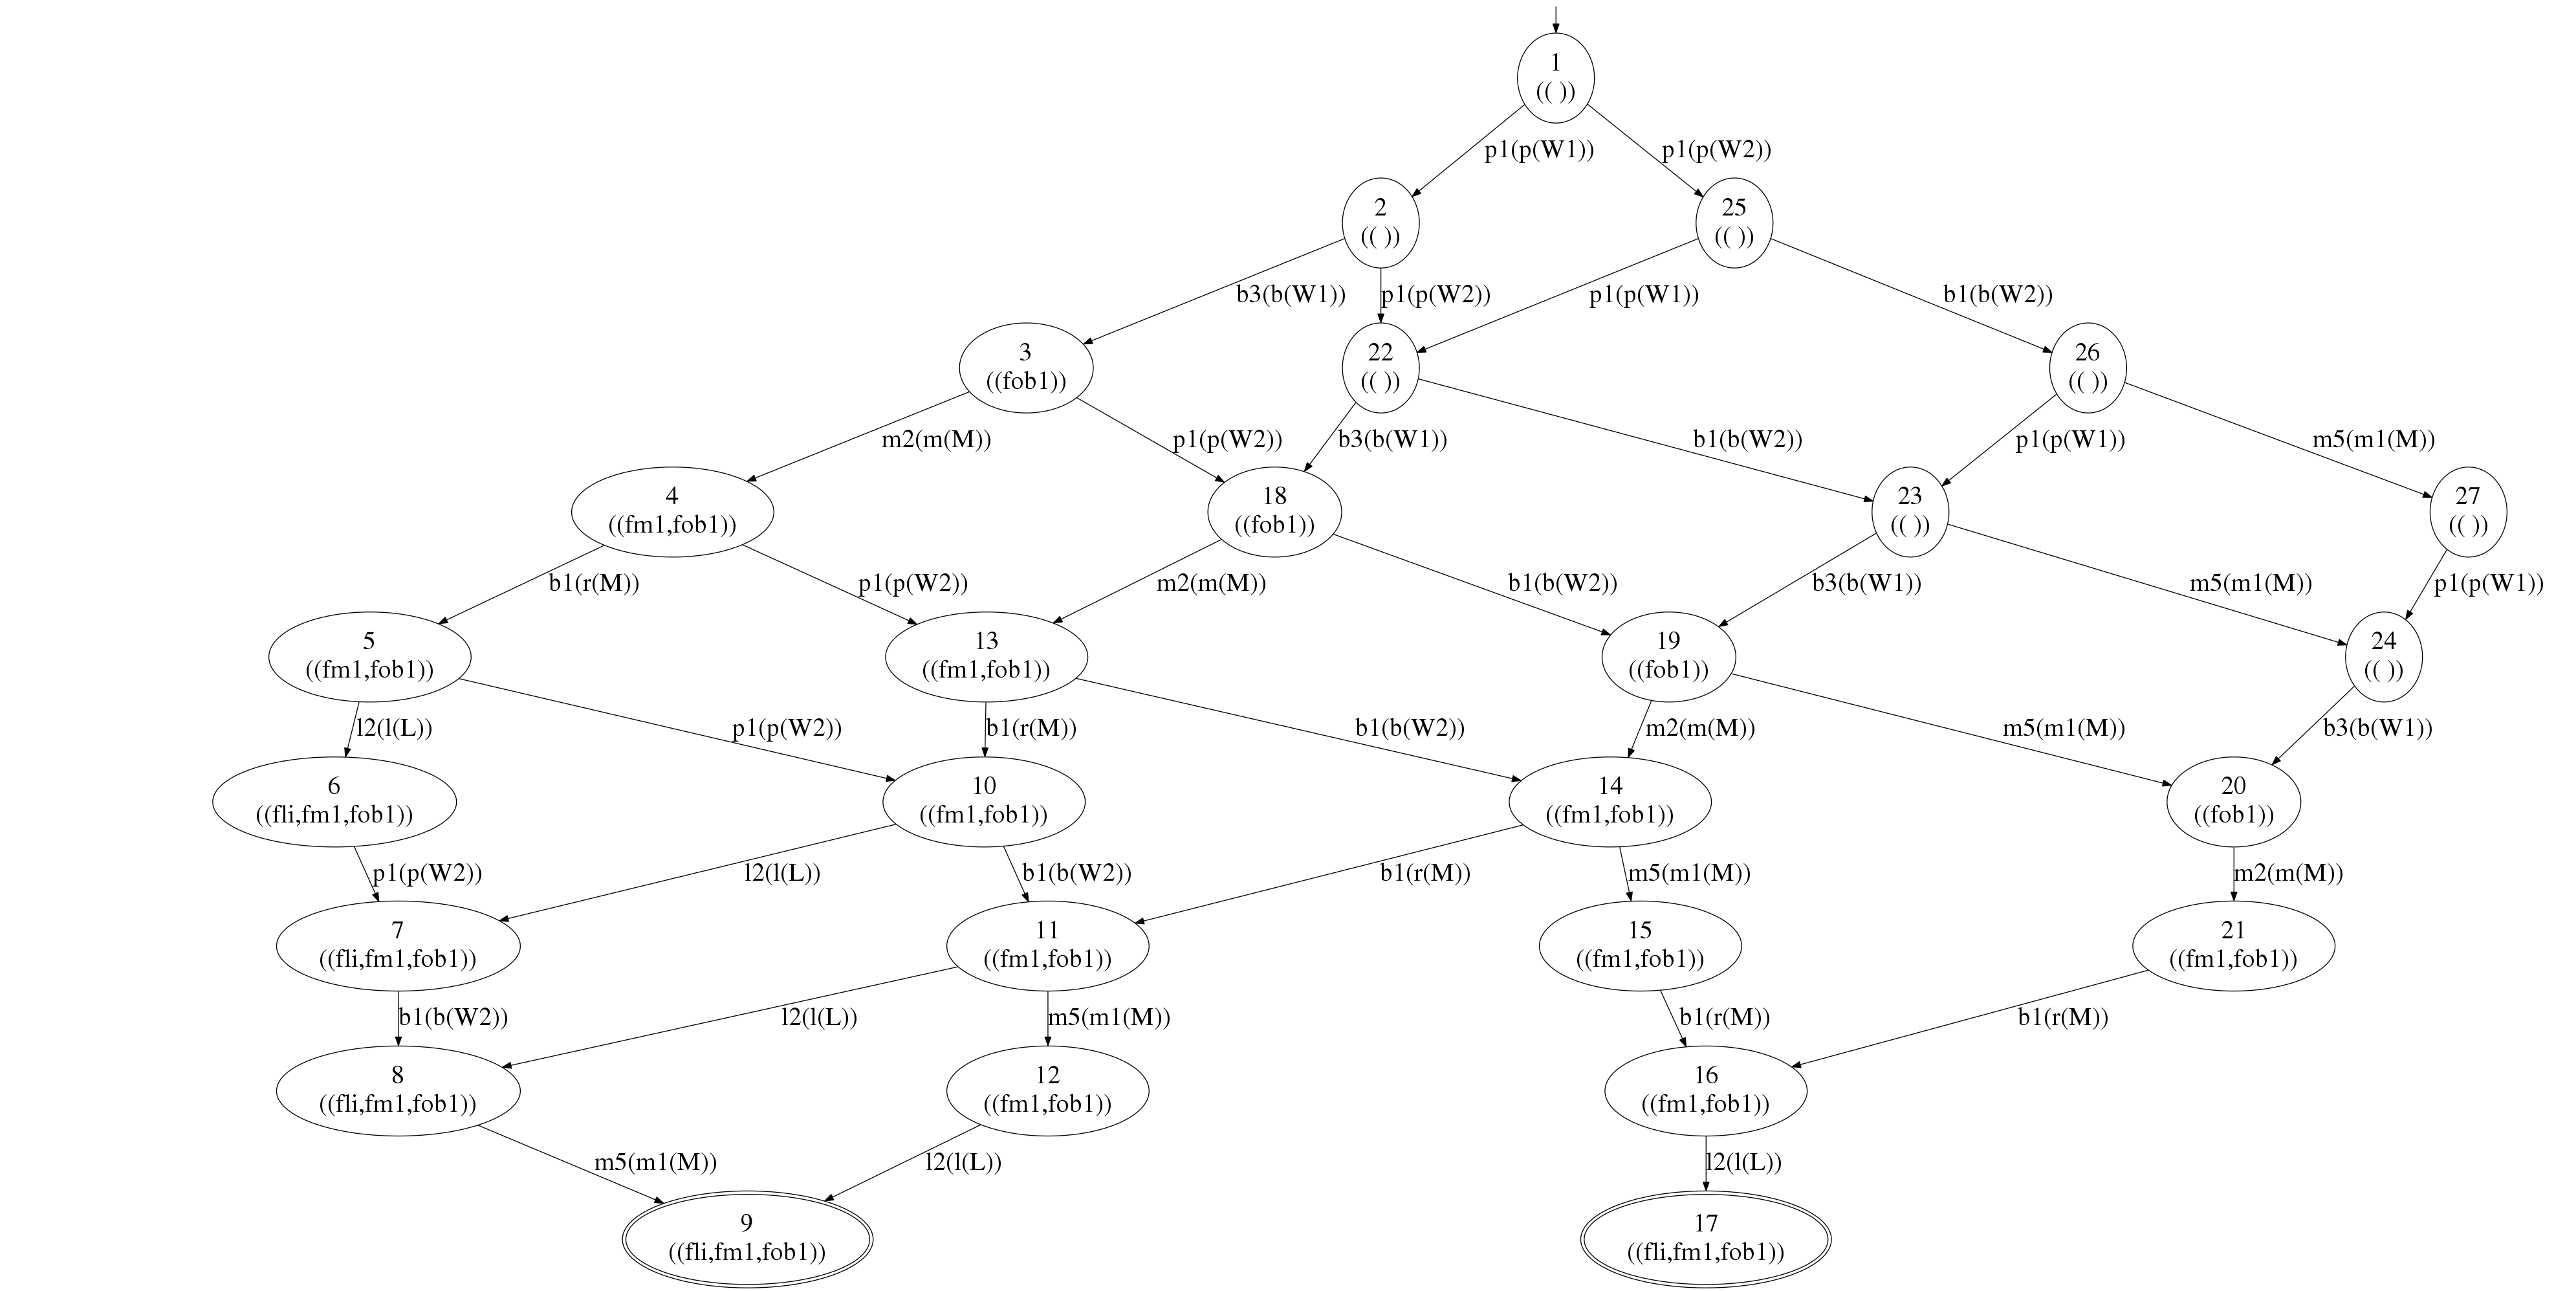
\includegraphics[scale=0.1]{./Img/sac/behavior.png}
\caption{Behavior del problema di riferimento}
\label{fig:bhv_c}
\end{figure}

\subsection{Distillazione delle diagnosi}
Una volta decorato il behavior, è possibile generare l'insieme delle soluzioni candidate esattamente come analizzato nel capitolo precedente.

\begin{ex}
Si consideri il behavior decorato in figura \ref{fig:bhv_c}. La soluzione del problema di diagnosi è data dall'unione delle diagnosi degli stati finali $9$ e $17$:
\begin{center}
$\Delta(P(\overline{C})) = \{\{fli,fm1,fob1\}\}$.
\end{center}
L'interpretazione di questo risultato è dovuto alla seguente dinamica:
\begin{itemize}
\item il breaker $b$ del nodo $W_1$ non si apre;
\item il monitor $m_1$ del nodo $M$, pur riuscendo a comandare l'apertura del proprio breaker di emergenza, fallisce nell'inviare il messaggio all'altro monitor;
\item la linea $l$ del nodo $L$, a fronte di un intervento di emergenza operato da un monitor, si trova isolata non potendo effettuare il ripristino.
\end{itemize}
\end{ex}

\newpage
\section{Diagnosi distribuita}
Il metodo di ricostruzione monolitica, analizzato nei paragrafi precedenti, è inefficiente in quanto la complessità della generazione del behavior dell'intero SAC è in generale esponenziale nel numero di componenti totali, nel numero di link, nel numero dei pattern space e nel numero dei nodi (ad ognuno dei quali corrisponde una sequenza di osservazione). Sebbene la ricostruzione permetta di non ricostruire il comportamento completo del sistema (behavior space), la ricostruzione del behavior è comunque costosa, sia in termini di tempo di esecuzione sia soprattutto di memoria.
Per questo motivo, nel corso di questo lavoro di tesi, è stato sviluppato un algoritmo distribuito che ricostruisce il comportamento del singolo nodo, unitamente alle informazioni necessarie scaturite dai pattern event, in modo da non dover generare il behavior del sistema nella sua interezza. Per fare questo si è seguita la topologia del sistema: trattandosi di una gerarchia, l'algoritmo opera in maniera bottom-up partendo dai nodi foglia. Il comportamento di questi ultimi, infatti, non è vincolato dal comportamento di nessun altro nodo, quindi la ricostruzione del loro comportamento è esattamente quella vista nel paragrafo precedente, eccetto il fatto che si considera il singolo nodo e non l'intero sistema. Per poter ricostruire i comportamenti dei nodi nel livello superiore della gerarchia, invece, è necessario considerare i pattern event che vengono inviati dal livello base. Per fare questo viene creata, per ogni nodo foglia, una interfaccia ottenuta togliendo dal linguaggio del behavior locale tutte quelle transizioni che non portano alla generazione di un pattern event in un terminale di uscita del nodo. I comportamenti del livello superiore, quindi, sono ricostruiti tenendo conto delle interfacce dei nodi sottostanti da cui essi dipendono. Ogni passaggio di stato dell'interfaccia sottostante corrisponde alla generazione di un pattern event che può essere consumato dai componenti a livello superiore. Il procedimento viene reiterato per ogni strato della gerarchia del sistema.
Una volta raggiunta la radice dell'albero, non è più necessario generare l'interfaccia di tale nodo (dato che nessun pattern event viene gestito da un livello superiore), quindi l'unico behavior corrispondente racchiude in sé tutte le diagnosi dell'intero sistema in forma sintetica. La sua decorazione permette di ricavare l'insieme di diagnosi candidate del SAC.

\subsection{Costruzione del Behavior non vincolato}
La ricostruzione dei behavior dei nodi foglia del SAC è un caso particolare della ricostruzione monolitica. Le variazioni consistono nel considerare solo i pattern space relativi al nodo locale e unicamente l'osservazione locale, la cui consumazione viene monitorata per mezzo di un unico indice di sequenza. Analogamente il viewer può essere ristretto al viewer locale del nodo corrente, in quanto si considerano solo transizioni di componenti appartenenti al nodo in esame.

\begin{ex}
In figura \ref{fig:bhv_leaves} sono riportati i behavior dei nodi foglia del problema di diagnosi di riferimento. Le transizioni e gli stati tratteggiati, al solito, costituiscono la parte spuria degli automi che non è in un cammino dallo stato iniziale ad uno stato finale.
Lo stato è descritto, in ordine, dagli stati della protezione e del breaker, dal contenuto del terminale di input del breaker, dallo stato corrente del pattern space (unico) del nodo e dall'indice della sequenza osservata del nodo. Si noti che le transizioni potrebbero essere identificate anche tralasciando il nodo di appartenenza. Tuttavia, per semplicità e conformità di notazione con i behavior vincolati, viene mantenuta anche questa informazione.
\end{ex}

\begin{figure}[htbp]
\centering
\subfigure[$Bhv(W1)$]
{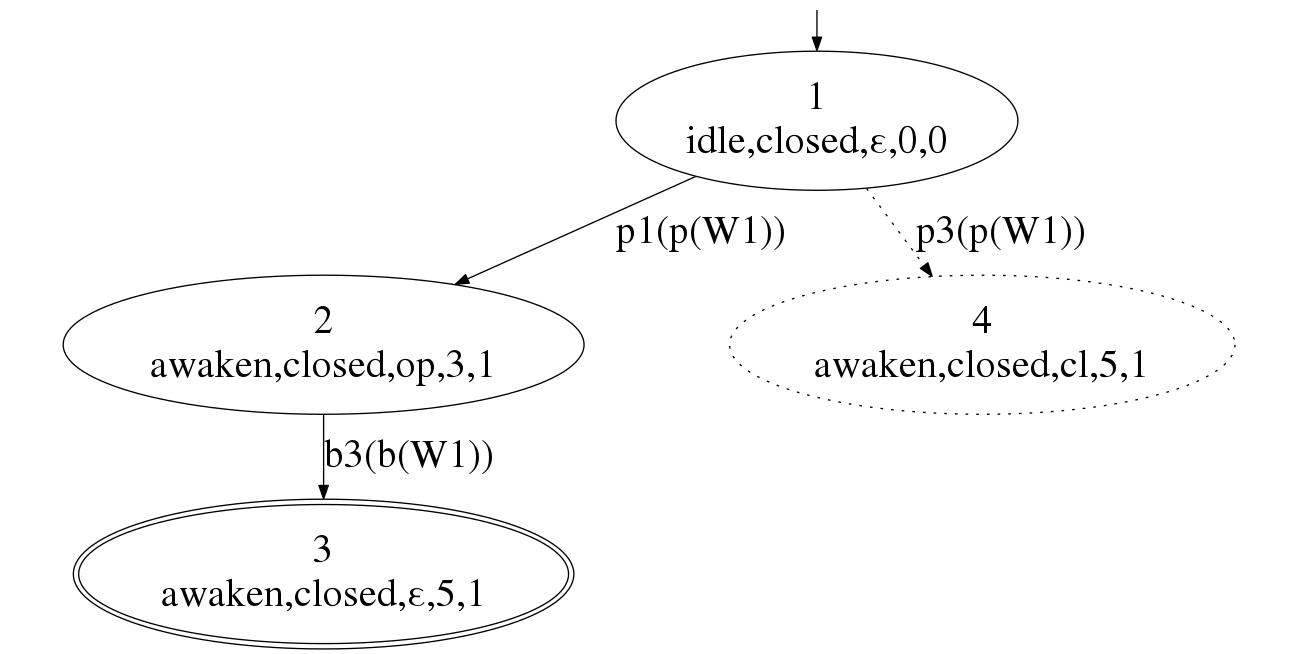
\includegraphics[scale=0.14]{./Img/sac/bhv_w1.png}}
\hspace{5mm}
\subfigure[$Bhv(W2)$]
{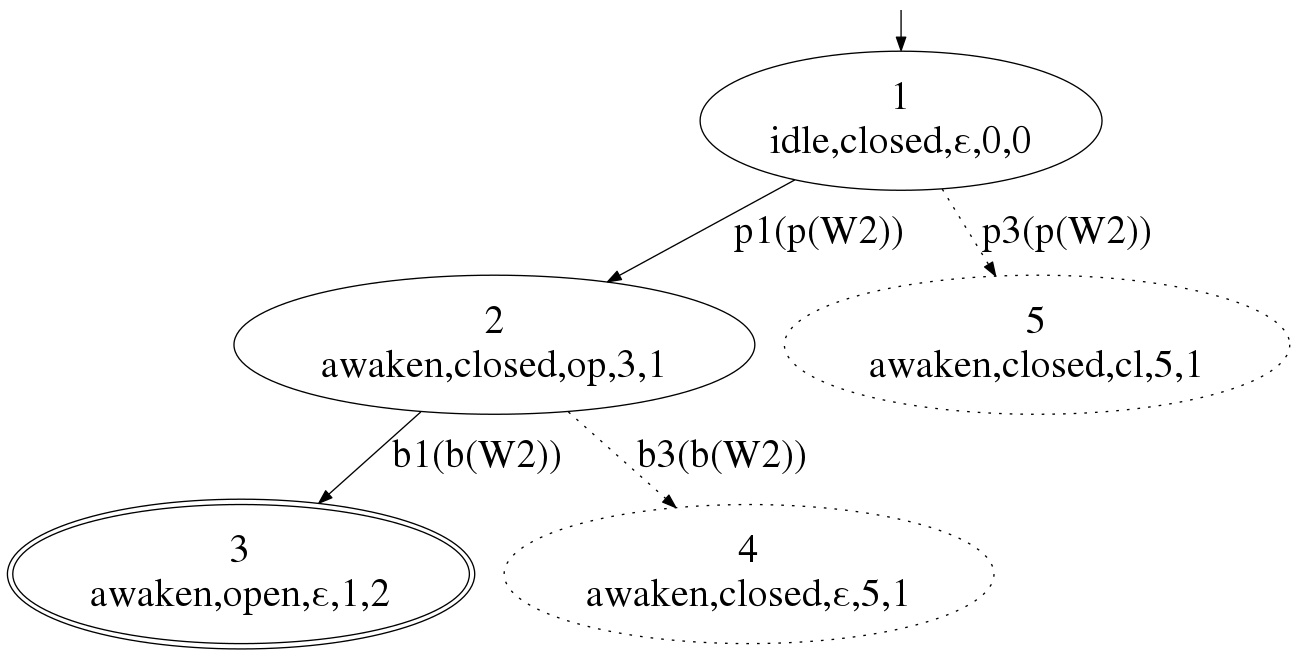
\includegraphics[scale=0.14]{./Img/sac/bhv_w2.png}}
\caption{Behavior dei nodi foglia $W1$ e $W2$}
\label{fig:bhv_leaves}
\end{figure}

\subsection{Generazione dell'interfaccia}
L'interfaccia di un nodo è un automa ottenuto eliminando dal linguaggio del behavior locale tutte le transizioni che non generano un pattern event.
La costruzione avviene come di seguito.
\begin{enumerate}
\item L'identificatore di una transizione di un componente $t(c)$ che provoca la generazione di un pattern event $(p,r,o)$ viene sostituito dal nome $p$ del pattern event generato, unitamente alla diagnosi relativa alla singola transizione che può essere:
\begin{itemize}
\item l'insieme singleton $\{\emptyset\}$ se la transizione è normale;
\item l'insieme singleton $\{\{f\}\}$, se la transizione è di guasto e $f$ è la corrispondente label associata nel ruler.
\end{itemize}
\item Le transizioni non associate ad alcun evento di pattern vengono interpretate come $\epsilon$-transizioni, ottenendo in questo modo un automa non deterministico (NFA). Quest'ultimo viene determinizzato attraverso un algoritmo simile alla subset construction: differisce da quest'ultima poichè la determinizzazione non si basa esclusivamente sui singoli stati del NFA, ma su tutta la sua struttura (pattern event e diagnosi relativa).
\end{enumerate}

\subsection{Costruzione del Behavior vincolato}
La costruzione del behavior vincolato riguarda tutti i nodi che non sono dei nodi foglia nella topologia del sistema. Per questo tipi di nodi, la ricostruzione del comportamento deve tenere conto delle informazioni aggiuntive riguardanti i pattern event che giungono dal livello inferiore. Questa informazione è racchiusa nelle interfacce dei nodi inferiori da cui il nodo corrente dipende. Un nodo dipende da un nodo di un livello inferiore se esiste un link che unisce un terminale di output da quel nodo inferiore al terminale di input del nodo in esame. Lo stato del behavior corrente, quindi, possiede l'informazione aggiuntava che riguarda la tupla di stati relativi alle interfacce da cui il nodo corrente dipende. Una transizione del comportamento può quindi essere di due tipi:
\begin{itemize}
\item una transizione $t(c)$ relativa ad un componente del nodo;
\item una transizione $t(Int)$ relativa ad una delle interfacce.
\end{itemize} 
Si noti che l'ultima è effettuabile se i link dove vengono generati i pattern event sono liberi (secondo la politica di saturazione wait adottata in questo lavoro).
Uno stato finale del behavior vincolato è tale se, oltre ad aver consumato completamente l'osservazione del nodo locale, ha raggiunto gli stati finali di tutte le interfacce da cui esso dipende. Quest'ultimo vincolo è necessario in quanto, proseguendo bottom-up nella ricostruzione, è necessario che ogni nodo abbia consumato la propria osservazione, affinché uno stato finale possa essere considerato il culmine di una traiettoria completa.

\subsection{Decorazione del Behavior del nodo radice}
Una volta che il metodo di ricostruzione distribuito raggiunge il nodo radice ed è stata effettuata la ricostruzione del behavior di quest'ultimo, è necessario effettuarne la decorazione, in maniera simile a quanto visto per il caso monolitico, con due variazioni:
\begin{itemize}
\item attraversando una transizione relativa a una interfaccia, è necessario combinare la diagnosi dello stato di partenza con la diagnosi associata alla transizione di interfaccia, mentre per le transizioni relative a componenti del nodo locale si mantiene il solito approccio, ricercando nel ruler se la transizione è presente e con quale label;
\item quando la decorazione raggiunge uno stato finale, bisogna combinare la diagnosi ottenute con la diagnosi relativa agli stati finali dell'interfaccia.
\end{itemize}
La seconda modifica è necessaria al fine di avere una diagnosi completa poiché, mentre negli stati non finali dell'interfaccia poi vi è una transizione che include le relative diagnosi contenute nello stato di partenza, in corrispondenza dello stato finale mancano le diagnosi di quello stato, che è finale e non necessita di dover percorrere ulteriori transizioni per raccoglierne le diagnosi.